% Options for packages loaded elsewhere
\PassOptionsToPackage{unicode}{hyperref}
\PassOptionsToPackage{hyphens}{url}
\PassOptionsToPackage{dvipsnames,svgnames,x11names}{xcolor}
%
\documentclass[
  letterpaper,
  DIV=11,
  numbers=noendperiod]{scrartcl}

\usepackage{amsmath,amssymb}
\usepackage{iftex}
\ifPDFTeX
  \usepackage[T1]{fontenc}
  \usepackage[utf8]{inputenc}
  \usepackage{textcomp} % provide euro and other symbols
\else % if luatex or xetex
  \usepackage{unicode-math}
  \defaultfontfeatures{Scale=MatchLowercase}
  \defaultfontfeatures[\rmfamily]{Ligatures=TeX,Scale=1}
\fi
\usepackage{lmodern}
\ifPDFTeX\else  
    % xetex/luatex font selection
\fi
% Use upquote if available, for straight quotes in verbatim environments
\IfFileExists{upquote.sty}{\usepackage{upquote}}{}
\IfFileExists{microtype.sty}{% use microtype if available
  \usepackage[]{microtype}
  \UseMicrotypeSet[protrusion]{basicmath} % disable protrusion for tt fonts
}{}
\makeatletter
\@ifundefined{KOMAClassName}{% if non-KOMA class
  \IfFileExists{parskip.sty}{%
    \usepackage{parskip}
  }{% else
    \setlength{\parindent}{0pt}
    \setlength{\parskip}{6pt plus 2pt minus 1pt}}
}{% if KOMA class
  \KOMAoptions{parskip=half}}
\makeatother
\usepackage{xcolor}
\setlength{\emergencystretch}{3em} % prevent overfull lines
\setcounter{secnumdepth}{-\maxdimen} % remove section numbering
% Make \paragraph and \subparagraph free-standing
\makeatletter
\ifx\paragraph\undefined\else
  \let\oldparagraph\paragraph
  \renewcommand{\paragraph}{
    \@ifstar
      \xxxParagraphStar
      \xxxParagraphNoStar
  }
  \newcommand{\xxxParagraphStar}[1]{\oldparagraph*{#1}\mbox{}}
  \newcommand{\xxxParagraphNoStar}[1]{\oldparagraph{#1}\mbox{}}
\fi
\ifx\subparagraph\undefined\else
  \let\oldsubparagraph\subparagraph
  \renewcommand{\subparagraph}{
    \@ifstar
      \xxxSubParagraphStar
      \xxxSubParagraphNoStar
  }
  \newcommand{\xxxSubParagraphStar}[1]{\oldsubparagraph*{#1}\mbox{}}
  \newcommand{\xxxSubParagraphNoStar}[1]{\oldsubparagraph{#1}\mbox{}}
\fi
\makeatother

\usepackage{color}
\usepackage{fancyvrb}
\newcommand{\VerbBar}{|}
\newcommand{\VERB}{\Verb[commandchars=\\\{\}]}
\DefineVerbatimEnvironment{Highlighting}{Verbatim}{commandchars=\\\{\}}
% Add ',fontsize=\small' for more characters per line
\usepackage{framed}
\definecolor{shadecolor}{RGB}{241,243,245}
\newenvironment{Shaded}{\begin{snugshade}}{\end{snugshade}}
\newcommand{\AlertTok}[1]{\textcolor[rgb]{0.68,0.00,0.00}{#1}}
\newcommand{\AnnotationTok}[1]{\textcolor[rgb]{0.37,0.37,0.37}{#1}}
\newcommand{\AttributeTok}[1]{\textcolor[rgb]{0.40,0.45,0.13}{#1}}
\newcommand{\BaseNTok}[1]{\textcolor[rgb]{0.68,0.00,0.00}{#1}}
\newcommand{\BuiltInTok}[1]{\textcolor[rgb]{0.00,0.23,0.31}{#1}}
\newcommand{\CharTok}[1]{\textcolor[rgb]{0.13,0.47,0.30}{#1}}
\newcommand{\CommentTok}[1]{\textcolor[rgb]{0.37,0.37,0.37}{#1}}
\newcommand{\CommentVarTok}[1]{\textcolor[rgb]{0.37,0.37,0.37}{\textit{#1}}}
\newcommand{\ConstantTok}[1]{\textcolor[rgb]{0.56,0.35,0.01}{#1}}
\newcommand{\ControlFlowTok}[1]{\textcolor[rgb]{0.00,0.23,0.31}{\textbf{#1}}}
\newcommand{\DataTypeTok}[1]{\textcolor[rgb]{0.68,0.00,0.00}{#1}}
\newcommand{\DecValTok}[1]{\textcolor[rgb]{0.68,0.00,0.00}{#1}}
\newcommand{\DocumentationTok}[1]{\textcolor[rgb]{0.37,0.37,0.37}{\textit{#1}}}
\newcommand{\ErrorTok}[1]{\textcolor[rgb]{0.68,0.00,0.00}{#1}}
\newcommand{\ExtensionTok}[1]{\textcolor[rgb]{0.00,0.23,0.31}{#1}}
\newcommand{\FloatTok}[1]{\textcolor[rgb]{0.68,0.00,0.00}{#1}}
\newcommand{\FunctionTok}[1]{\textcolor[rgb]{0.28,0.35,0.67}{#1}}
\newcommand{\ImportTok}[1]{\textcolor[rgb]{0.00,0.46,0.62}{#1}}
\newcommand{\InformationTok}[1]{\textcolor[rgb]{0.37,0.37,0.37}{#1}}
\newcommand{\KeywordTok}[1]{\textcolor[rgb]{0.00,0.23,0.31}{\textbf{#1}}}
\newcommand{\NormalTok}[1]{\textcolor[rgb]{0.00,0.23,0.31}{#1}}
\newcommand{\OperatorTok}[1]{\textcolor[rgb]{0.37,0.37,0.37}{#1}}
\newcommand{\OtherTok}[1]{\textcolor[rgb]{0.00,0.23,0.31}{#1}}
\newcommand{\PreprocessorTok}[1]{\textcolor[rgb]{0.68,0.00,0.00}{#1}}
\newcommand{\RegionMarkerTok}[1]{\textcolor[rgb]{0.00,0.23,0.31}{#1}}
\newcommand{\SpecialCharTok}[1]{\textcolor[rgb]{0.37,0.37,0.37}{#1}}
\newcommand{\SpecialStringTok}[1]{\textcolor[rgb]{0.13,0.47,0.30}{#1}}
\newcommand{\StringTok}[1]{\textcolor[rgb]{0.13,0.47,0.30}{#1}}
\newcommand{\VariableTok}[1]{\textcolor[rgb]{0.07,0.07,0.07}{#1}}
\newcommand{\VerbatimStringTok}[1]{\textcolor[rgb]{0.13,0.47,0.30}{#1}}
\newcommand{\WarningTok}[1]{\textcolor[rgb]{0.37,0.37,0.37}{\textit{#1}}}

\providecommand{\tightlist}{%
  \setlength{\itemsep}{0pt}\setlength{\parskip}{0pt}}\usepackage{longtable,booktabs,array}
\usepackage{calc} % for calculating minipage widths
% Correct order of tables after \paragraph or \subparagraph
\usepackage{etoolbox}
\makeatletter
\patchcmd\longtable{\par}{\if@noskipsec\mbox{}\fi\par}{}{}
\makeatother
% Allow footnotes in longtable head/foot
\IfFileExists{footnotehyper.sty}{\usepackage{footnotehyper}}{\usepackage{footnote}}
\makesavenoteenv{longtable}
\usepackage{graphicx}
\makeatletter
\def\maxwidth{\ifdim\Gin@nat@width>\linewidth\linewidth\else\Gin@nat@width\fi}
\def\maxheight{\ifdim\Gin@nat@height>\textheight\textheight\else\Gin@nat@height\fi}
\makeatother
% Scale images if necessary, so that they will not overflow the page
% margins by default, and it is still possible to overwrite the defaults
% using explicit options in \includegraphics[width, height, ...]{}
\setkeys{Gin}{width=\maxwidth,height=\maxheight,keepaspectratio}
% Set default figure placement to htbp
\makeatletter
\def\fps@figure{htbp}
\makeatother

\usepackage{fvextra}
\DefineVerbatimEnvironment{Highlighting}{Verbatim}{breaklines,commandchars=\\\{\}}
\KOMAoption{captions}{tableheading}
\makeatletter
\@ifpackageloaded{caption}{}{\usepackage{caption}}
\AtBeginDocument{%
\ifdefined\contentsname
  \renewcommand*\contentsname{Table of contents}
\else
  \newcommand\contentsname{Table of contents}
\fi
\ifdefined\listfigurename
  \renewcommand*\listfigurename{List of Figures}
\else
  \newcommand\listfigurename{List of Figures}
\fi
\ifdefined\listtablename
  \renewcommand*\listtablename{List of Tables}
\else
  \newcommand\listtablename{List of Tables}
\fi
\ifdefined\figurename
  \renewcommand*\figurename{Figure}
\else
  \newcommand\figurename{Figure}
\fi
\ifdefined\tablename
  \renewcommand*\tablename{Table}
\else
  \newcommand\tablename{Table}
\fi
}
\@ifpackageloaded{float}{}{\usepackage{float}}
\floatstyle{ruled}
\@ifundefined{c@chapter}{\newfloat{codelisting}{h}{lop}}{\newfloat{codelisting}{h}{lop}[chapter]}
\floatname{codelisting}{Listing}
\newcommand*\listoflistings{\listof{codelisting}{List of Listings}}
\makeatother
\makeatletter
\makeatother
\makeatletter
\@ifpackageloaded{caption}{}{\usepackage{caption}}
\@ifpackageloaded{subcaption}{}{\usepackage{subcaption}}
\makeatother

\ifLuaTeX
  \usepackage{selnolig}  % disable illegal ligatures
\fi
\usepackage{bookmark}

\IfFileExists{xurl.sty}{\usepackage{xurl}}{} % add URL line breaks if available
\urlstyle{same} % disable monospaced font for URLs
\hypersetup{
  pdftitle={PS4: Spatial},
  pdfauthor={Hiroaki Kurachi, Luis Senires},
  colorlinks=true,
  linkcolor={blue},
  filecolor={Maroon},
  citecolor={Blue},
  urlcolor={Blue},
  pdfcreator={LaTeX via pandoc}}


\title{PS4: Spatial}
\author{Hiroaki Kurachi, Luis Senires}
\date{2024-11-03}

\begin{document}
\maketitle

\RecustomVerbatimEnvironment{verbatim}{Verbatim}{
  showspaces = false,
  showtabs = false,
  breaksymbolleft={},
  breaklines
}


\textbf{PS4:} Due Sat Nov 2 at 5:00PM Central. Worth 100 points. We use
(\texttt{*}) to indicate a problem that we think might be time
consuming.

\subsection{Style Points (10 pts)}\label{style-points-10-pts}

\subsection{Submission Steps (10 pts)}\label{submission-steps-10-pts}

\begin{enumerate}
\def\labelenumi{\arabic{enumi}.}
\item
  This problem set is a paired problem set.
\item
  Play paper, scissors, rock to determine who goes first. Call that
  person Partner 1.
\end{enumerate}

• Partner 1 (Hiroaki Kurachi and hiroakik):

• Partner 2 (Luis Senires and ldsenires):

\begin{enumerate}
\def\labelenumi{\arabic{enumi}.}
\setcounter{enumi}{2}
\item
  Partner 1 will accept the ps4 and then share the link it creates with
  their partner. You can only share it with one partner so you will not
  be able to change it after your partner has accepted.
\item
  ``This submission is our work alone and complies with the 30538
  integrity policy.'' Add your initials to indicate your agreement:
  \textbf{HK} \textbf{LS}
\item
  ``I have uploaded the names of anyone else other than my partner and I
  worked with on the problem set here'' (1 point)
\item
  Late coins used this pset: \textbf{01} Late coins left after
  submission: \textbf{02}
\item
  Knit your ps4.qmd to an PDF file to make ps4.pdf,
\end{enumerate}

• The PDF should not be more than 25 pages. Use head() and re-size
figures when appropriate.

\begin{enumerate}
\def\labelenumi{\arabic{enumi}.}
\setcounter{enumi}{7}
\item
  (Partner 1): push ps4.qmd and ps4.pdf to your github repo.
\item
  (Partner 1): submit ps4.pdf via Gradescope. Add your partner on
  Gradescope.
\item
  (Partner 1): tag your submission in Gradescope
\end{enumerate}

\begin{Shaded}
\begin{Highlighting}[]
\ImportTok{import}\NormalTok{ os}
\ImportTok{import}\NormalTok{ pandas }\ImportTok{as}\NormalTok{ pd}
\ImportTok{import}\NormalTok{ altair }\ImportTok{as}\NormalTok{ alt}
\ImportTok{import}\NormalTok{ geopandas }\ImportTok{as}\NormalTok{ gpd}
\ImportTok{import}\NormalTok{ matplotlib.pyplot }\ImportTok{as}\NormalTok{ plt}
\ImportTok{import}\NormalTok{ numpy }\ImportTok{as}\NormalTok{ np}
\ImportTok{import}\NormalTok{ time}
\ImportTok{import}\NormalTok{ datetime }\ImportTok{as}\NormalTok{ datetime}

\ImportTok{import}\NormalTok{ warnings}
\NormalTok{warnings.filterwarnings(}\StringTok{\textquotesingle{}ignore\textquotesingle{}}\NormalTok{)}
\end{Highlighting}
\end{Shaded}

\subsection{Download and explore the Provider of Services (POS) file (10
pts)}\label{download-and-explore-the-provider-of-services-pos-file-10-pts}

\begin{enumerate}
\def\labelenumi{\arabic{enumi}.}
\tightlist
\item
\end{enumerate}

The variables we selected are;

\begin{itemize}
\item
  PRVDR\_NUM: CMS certification number
\item
  PRVDR\_CTGRY\_CD: the type of provider participating in the
  Medicare/Medicaid program
\item
  PRVDR\_CTGRY\_SBTYP\_CD: the subtype of the provider, within the
  primary category
\item
  FAC\_NAME: name of the provider certified to participate in the
  Medicare and/or Medicaid programs
\item
  CITY\_NAME: city in which the provider is physically located
\item
  ST\_ADR: street address where the provider is located
\item
  ZIP\_CD; five-digit ZIP code for a provider's physical address
\item
  TRMNTN\_EXPRTN\_DT: date the provider was terminated
\item
  PGM\_TRMNTN\_CD: indicates the current termination status for the
  provider
\end{itemize}

\begin{enumerate}
\def\labelenumi{\arabic{enumi}.}
\setcounter{enumi}{1}
\tightlist
\item
\end{enumerate}

\begin{Shaded}
\begin{Highlighting}[]
\CommentTok{\# Set the absolute path of the data folder}
\CommentTok{\# base = (r"C:\textbackslash{}Users\textbackslash{}hkura\textbackslash{}Documents\textbackslash{}Uchicago\textbackslash{}04 2024 Autumn\textbackslash{}Python2\textbackslash{}problem{-}set{-}4{-}hiro{-}luis\textbackslash{}data")}
\NormalTok{base }\OperatorTok{=}\NormalTok{ (}\VerbatimStringTok{r"C:\textbackslash{}Users\textbackslash{}LUIS\textbackslash{}Documents\textbackslash{}GitHub\textbackslash{}problem{-}set{-}4{-}hiro{-}luis\textbackslash{}data"}\NormalTok{)}
\NormalTok{path\_data\_2016 }\OperatorTok{=}\NormalTok{ os.path.join(base, }\StringTok{"pos2016.csv"}\NormalTok{)}

\CommentTok{\# Load 2016 dataset}
\NormalTok{df\_pos2016 }\OperatorTok{=}\NormalTok{ pd.read\_csv(path\_data\_2016, encoding}\OperatorTok{=}\StringTok{"utf{-}8"}\NormalTok{)}

\CommentTok{\# Define function to subset a dataset for short{-}term hospitals}


\KeywordTok{def}\NormalTok{ subset\_short\_term(df):}
\NormalTok{    df\_result }\OperatorTok{=}\NormalTok{ df[(df[}\StringTok{"PRVDR\_CTGRY\_CD"}\NormalTok{] }\OperatorTok{==} \DecValTok{1}\NormalTok{) }\OperatorTok{\&}
\NormalTok{                   (df[}\StringTok{"PRVDR\_CTGRY\_SBTYP\_CD"}\NormalTok{] }\OperatorTok{==} \DecValTok{1}\NormalTok{)]}
    \ControlFlowTok{return}\NormalTok{ df\_result}


\CommentTok{\# Create short{-}term hospitals subsets for 2016 dataset}
\NormalTok{df\_pos2016\_short }\OperatorTok{=}\NormalTok{ subset\_short\_term(df\_pos2016)}
\end{Highlighting}
\end{Shaded}

\begin{verbatim}
a.    
\end{verbatim}

\begin{Shaded}
\begin{Highlighting}[]
\CommentTok{\# Count the number of observations}
\BuiltInTok{print}\NormalTok{(}\BuiltInTok{len}\NormalTok{(df\_pos2016\_short))}
\end{Highlighting}
\end{Shaded}

\begin{verbatim}
7245
\end{verbatim}

\begin{verbatim}
This subset for short-term hospitals in 2016 includes 7245 hospitals.

This number seems not making sense, as it occupies a half of number of whole hospitals though it is just one subtype. 
\end{verbatim}

\begin{Shaded}
\begin{Highlighting}[]
\CommentTok{\# Count the number of observations}
\BuiltInTok{print}\NormalTok{(}\BuiltInTok{len}\NormalTok{(df\_pos2016))}
\end{Highlighting}
\end{Shaded}

\begin{verbatim}
141557
\end{verbatim}

\begin{verbatim}
b. We couldn't find references which includes the exact number of short-term hospitals at the end of 2016, but the 2016 CMS statistics specifies the number as 3,436 for the Dec 31, 2015, which is the most recent data available in the search result(https://www.cms.gov/Research-Statistics-Data-and-Systems/Statistics-
Trends-and-Reports/CMS-Statistics-Reference-Booklet/
Downloads/2016_CMS_Stats.pdf).

Considering the number 3,436 at the end of 2015, 7245 is drastically larger, even considering the change in one year.

As far as we could find, there seems no substantial policy change in 2016, which could potentially change the number of healthcare providers drastically.

As both the dataset we use and the cross-reference are both published by Centers for Medicare & Medicaid Services, it might be plausible to assume their credibilities. And as the dataset dictionary says nothing about change in definition of the provider categories/sub-categories. Then one reason we can consider is, for instance, the change in the data gathering methods. 
\end{verbatim}

\begin{enumerate}
\def\labelenumi{\arabic{enumi}.}
\setcounter{enumi}{2}
\tightlist
\item
\end{enumerate}

\begin{Shaded}
\begin{Highlighting}[]
\CommentTok{\# Load 2017{-}2019 datasets}
\NormalTok{path\_data\_2017 }\OperatorTok{=}\NormalTok{ os.path.join(base, }\StringTok{"pos2017.csv"}\NormalTok{)}
\NormalTok{path\_data\_2018 }\OperatorTok{=}\NormalTok{ os.path.join(base, }\StringTok{"pos2018.csv"}\NormalTok{)}
\NormalTok{path\_data\_2019 }\OperatorTok{=}\NormalTok{ os.path.join(base, }\StringTok{"pos2019.csv"}\NormalTok{)}
\NormalTok{df\_pos2017 }\OperatorTok{=}\NormalTok{ pd.read\_csv(path\_data\_2017, encoding}\OperatorTok{=}\StringTok{"utf{-}8"}\NormalTok{)}
\NormalTok{df\_pos2018 }\OperatorTok{=}\NormalTok{ pd.read\_csv(path\_data\_2018, encoding}\OperatorTok{=}\StringTok{"latin1"}\NormalTok{)}
\NormalTok{df\_pos2019 }\OperatorTok{=}\NormalTok{ pd.read\_csv(path\_data\_2019, encoding}\OperatorTok{=}\StringTok{"latin1"}\NormalTok{)}

\CommentTok{\# Clean 2018, 2019 datasets: fix colname}


\KeywordTok{def}\NormalTok{ fix\_col(df):}
\NormalTok{    col }\OperatorTok{=}\NormalTok{ df.columns.tolist()}
\NormalTok{    col[}\DecValTok{0}\NormalTok{] }\OperatorTok{=} \StringTok{"PRVDR\_NUM"}
\NormalTok{    df.columns }\OperatorTok{=}\NormalTok{ col}
    \ControlFlowTok{return}\NormalTok{ df}


\NormalTok{df\_pos2018 }\OperatorTok{=}\NormalTok{ fix\_col(df\_pos2018)}
\NormalTok{df\_pos2019 }\OperatorTok{=}\NormalTok{ fix\_col(df\_pos2019)}

\CommentTok{\# Create short{-}term hospitals subsets for 2017{-}2019 datasets}
\NormalTok{df\_pos2017\_short }\OperatorTok{=}\NormalTok{ subset\_short\_term(df\_pos2017)}
\NormalTok{df\_pos2018\_short }\OperatorTok{=}\NormalTok{ subset\_short\_term(df\_pos2018)}
\NormalTok{df\_pos2019\_short }\OperatorTok{=}\NormalTok{ subset\_short\_term(df\_pos2019)}


\CommentTok{\# Summarize the number of observations for each subset}
\NormalTok{df\_summary\_obs }\OperatorTok{=}\NormalTok{ pd.DataFrame(}
\NormalTok{    \{}\StringTok{"year"}\NormalTok{: }\BuiltInTok{list}\NormalTok{(}\BuiltInTok{range}\NormalTok{(}\DecValTok{2016}\NormalTok{, }\DecValTok{2020}\NormalTok{, }\DecValTok{1}\NormalTok{)),}
     \StringTok{"observations"}\NormalTok{: [}\BuiltInTok{len}\NormalTok{(df\_pos2016\_short), }\BuiltInTok{len}\NormalTok{(df\_pos2017\_short), }\BuiltInTok{len}\NormalTok{(df\_pos2018\_short), }\BuiltInTok{len}\NormalTok{(df\_pos2019\_short)]}
\NormalTok{     \}}
\NormalTok{)}

\NormalTok{df\_summary\_obs}
\end{Highlighting}
\end{Shaded}

\begin{longtable}[]{@{}lll@{}}
\toprule\noalign{}
& year & observations \\
\midrule\noalign{}
\endhead
\bottomrule\noalign{}
\endlastfoot
0 & 2016 & 7245 \\
1 & 2017 & 7260 \\
2 & 2018 & 7277 \\
3 & 2019 & 7303 \\
\end{longtable}

The number for q4 in 2017/2018/2019 is on similar level with 2016, which
are unmatched with the cross-reference.

\begin{Shaded}
\begin{Highlighting}[]
\CommentTok{\# Add "DATA\_YEAR" column to each subsets}
\NormalTok{df\_pos2016\_short[}\StringTok{"DATA\_YEAR"}\NormalTok{] }\OperatorTok{=} \DecValTok{2016}
\NormalTok{df\_pos2017\_short[}\StringTok{"DATA\_YEAR"}\NormalTok{] }\OperatorTok{=} \DecValTok{2017}
\NormalTok{df\_pos2018\_short[}\StringTok{"DATA\_YEAR"}\NormalTok{] }\OperatorTok{=} \DecValTok{2018}
\NormalTok{df\_pos2019\_short[}\StringTok{"DATA\_YEAR"}\NormalTok{] }\OperatorTok{=} \DecValTok{2019}

\CommentTok{\# Concaterate the subsets}
\NormalTok{df\_pos\_append }\OperatorTok{=}\NormalTok{ pd.concat(}
\NormalTok{    [df\_pos2016\_short, df\_pos2017\_short, df\_pos2018\_short, df\_pos2019\_short])}

\CommentTok{\# Turn off the row number limit}
\NormalTok{alt.data\_transformers.disable\_max\_rows()}

\CommentTok{\# Plot the number of observation for each subset\textquotesingle{}s year}
\NormalTok{chart\_obs }\OperatorTok{=}\NormalTok{ alt.Chart(df\_pos\_append).mark\_line().encode(}
\NormalTok{    alt.X(}\StringTok{"DATA\_YEAR:N"}\NormalTok{, title}\OperatorTok{=}\StringTok{"Year (Q4)"}\NormalTok{, axis}\OperatorTok{=}\NormalTok{alt.Axis(labelAngle}\OperatorTok{=}\DecValTok{0}\NormalTok{)),}
\NormalTok{    alt.Y(}\StringTok{"count()"}\NormalTok{, title}\OperatorTok{=}\StringTok{"Number of Observation"}\NormalTok{,}
\NormalTok{          scale}\OperatorTok{=}\NormalTok{alt.Scale(domain}\OperatorTok{=}\NormalTok{[}\DecValTok{7000}\NormalTok{, }\DecValTok{8000}\NormalTok{]))}
\NormalTok{).properties(width}\OperatorTok{=}\DecValTok{250}\NormalTok{, height}\OperatorTok{=}\DecValTok{250}\NormalTok{)}
\NormalTok{chart\_obs}
\end{Highlighting}
\end{Shaded}

\begin{verbatim}
alt.Chart(...)
\end{verbatim}

\begin{enumerate}
\def\labelenumi{\arabic{enumi}.}
\setcounter{enumi}{3}
\tightlist
\item
  \begin{enumerate}
  \def\labelenumii{\alph{enumii}.}
  \tightlist
  \item
  \end{enumerate}
\end{enumerate}

\begin{Shaded}
\begin{Highlighting}[]
\CommentTok{\# Summarize the number of unique providers for each subset}
\NormalTok{df\_summary\_unique }\OperatorTok{=}\NormalTok{ pd.DataFrame(}
\NormalTok{    \{}\StringTok{"year"}\NormalTok{: }\BuiltInTok{list}\NormalTok{(}\BuiltInTok{range}\NormalTok{(}\DecValTok{2016}\NormalTok{, }\DecValTok{2020}\NormalTok{, }\DecValTok{1}\NormalTok{)),}
     \StringTok{"unique\_hospitals"}\NormalTok{:  [}\BuiltInTok{len}\NormalTok{(df\_pos2016\_short[}\StringTok{"PRVDR\_NUM"}\NormalTok{].value\_counts()), }\BuiltInTok{len}\NormalTok{(df\_pos2017\_short[}\StringTok{"PRVDR\_NUM"}\NormalTok{].value\_counts()), }\BuiltInTok{len}\NormalTok{(df\_pos2018\_short[}\StringTok{"PRVDR\_NUM"}\NormalTok{].value\_counts()), }\BuiltInTok{len}\NormalTok{(df\_pos2019\_short[}\StringTok{"PRVDR\_NUM"}\NormalTok{].value\_counts())]}
\NormalTok{     \}}
\NormalTok{)}

\NormalTok{df\_summary\_unique}

\CommentTok{\# Plot the number of unique hospitals for each subset\textquotesingle{}s year}
\NormalTok{chart\_unique }\OperatorTok{=}\NormalTok{ alt.Chart(df\_summary\_unique).mark\_line().encode(}
\NormalTok{    alt.X(}\StringTok{"year:N"}\NormalTok{, title}\OperatorTok{=}\StringTok{"Year (Q4)"}\NormalTok{, axis}\OperatorTok{=}\NormalTok{alt.Axis(labelAngle}\OperatorTok{=}\DecValTok{0}\NormalTok{)),}
\NormalTok{    alt.Y(}\StringTok{"unique\_hospitals:Q"}\NormalTok{, title}\OperatorTok{=}\StringTok{"Number of unique hospitals"}\NormalTok{,}
\NormalTok{          scale}\OperatorTok{=}\NormalTok{alt.Scale(domain}\OperatorTok{=}\NormalTok{[}\DecValTok{7000}\NormalTok{, }\DecValTok{8000}\NormalTok{]))}
\NormalTok{).properties(width}\OperatorTok{=}\DecValTok{250}\NormalTok{, height}\OperatorTok{=}\DecValTok{250}\NormalTok{)}
\NormalTok{chart\_unique}
\end{Highlighting}
\end{Shaded}

\begin{verbatim}
alt.Chart(...)
\end{verbatim}

\begin{verbatim}
b.
The numbers of unique hospitals are the same as the numbers of observations for all years we examined. This suggests that this dataset is structured so that each row contains parameters/attributions of each hospital.
\end{verbatim}

\subsection{Identify hospital closures in POS file (15 pts)
(*)}\label{identify-hospital-closures-in-pos-file-15-pts}

\begin{enumerate}
\def\labelenumi{\arabic{enumi}.}
\tightlist
\item
\end{enumerate}

\begin{Shaded}
\begin{Highlighting}[]
\CommentTok{\# Make termination status per year a separate column}
\NormalTok{df\_pos2016\_short.rename(}
\NormalTok{    columns}\OperatorTok{=}\NormalTok{\{}\StringTok{"PGM\_TRMNTN\_CD"}\NormalTok{: }\StringTok{"PGM\_TRMNTN\_CD\_2016"}\NormalTok{\}, inplace}\OperatorTok{=}\VariableTok{True}\NormalTok{)}
\NormalTok{df\_pos2017\_short.rename(}
\NormalTok{    columns}\OperatorTok{=}\NormalTok{\{}\StringTok{"PGM\_TRMNTN\_CD"}\NormalTok{: }\StringTok{"PGM\_TRMNTN\_CD\_2017"}\NormalTok{\}, inplace}\OperatorTok{=}\VariableTok{True}\NormalTok{)}
\NormalTok{df\_pos2018\_short.rename(}
\NormalTok{    columns}\OperatorTok{=}\NormalTok{\{}\StringTok{"PGM\_TRMNTN\_CD"}\NormalTok{: }\StringTok{"PGM\_TRMNTN\_CD\_2018"}\NormalTok{\}, inplace}\OperatorTok{=}\VariableTok{True}\NormalTok{)}
\NormalTok{df\_pos2019\_short.rename(}
\NormalTok{    columns}\OperatorTok{=}\NormalTok{\{}\StringTok{"PGM\_TRMNTN\_CD"}\NormalTok{: }\StringTok{"PGM\_TRMNTN\_CD\_2019"}\NormalTok{\}, inplace}\OperatorTok{=}\VariableTok{True}\NormalTok{)}
\end{Highlighting}
\end{Shaded}

\begin{Shaded}
\begin{Highlighting}[]
\CommentTok{\# Create new merged df}
\NormalTok{df\_list }\OperatorTok{=}\NormalTok{ [df\_pos2017\_short, df\_pos2018\_short, df\_pos2019\_short]}
\NormalTok{df\_pos\_termination }\OperatorTok{=}\NormalTok{ df\_pos2016\_short}

\ControlFlowTok{for}\NormalTok{ df }\KeywordTok{in}\NormalTok{ df\_list:}
\NormalTok{    col\_name }\OperatorTok{=}\NormalTok{ df.columns[}\OperatorTok{{-}}\DecValTok{2}\NormalTok{]}
\NormalTok{    df\_pos\_termination }\OperatorTok{=}\NormalTok{ df\_pos\_termination.merge(}
\NormalTok{        df[[}\StringTok{"PRVDR\_NUM"}\NormalTok{, col\_name]], on}\OperatorTok{=}\StringTok{"PRVDR\_NUM"}\NormalTok{, how}\OperatorTok{=}\StringTok{"outer"}\NormalTok{)}

\NormalTok{df\_pos\_termination }\OperatorTok{=}\NormalTok{ df\_pos\_termination.drop(columns}\OperatorTok{=}\NormalTok{[}\StringTok{"DATA\_YEAR"}\NormalTok{])}
\end{Highlighting}
\end{Shaded}

\begin{Shaded}
\begin{Highlighting}[]
\CommentTok{\# Add suspected termination year}
\KeywordTok{def}\NormalTok{ add\_termination\_year(row):}
    \ControlFlowTok{if}\NormalTok{ row[}\StringTok{"PGM\_TRMNTN\_CD\_2016"}\NormalTok{] }\OperatorTok{!=} \DecValTok{0}\NormalTok{:}
        \ControlFlowTok{return} \VariableTok{None}
    \ControlFlowTok{elif}\NormalTok{ row[}\StringTok{"PGM\_TRMNTN\_CD\_2017"}\NormalTok{] }\OperatorTok{!=} \DecValTok{0}\NormalTok{:}
        \ControlFlowTok{return} \DecValTok{2017}
    \ControlFlowTok{elif}\NormalTok{ row[}\StringTok{"PGM\_TRMNTN\_CD\_2018"}\NormalTok{] }\OperatorTok{!=} \DecValTok{0}\NormalTok{:}
        \ControlFlowTok{return} \DecValTok{2018}
    \ControlFlowTok{elif}\NormalTok{ row[}\StringTok{"PGM\_TRMNTN\_CD\_2019"}\NormalTok{] }\OperatorTok{!=} \DecValTok{0}\NormalTok{:}
        \ControlFlowTok{return} \DecValTok{2019}
    \ControlFlowTok{return} \VariableTok{None}


\NormalTok{df\_pos\_termination[}\StringTok{"TRMNTN\_YEAR"}\NormalTok{] }\OperatorTok{=}\NormalTok{ df\_pos\_termination.}\BuiltInTok{apply}\NormalTok{(}
\NormalTok{    add\_termination\_year, axis}\OperatorTok{=}\DecValTok{1}\NormalTok{)}
\end{Highlighting}
\end{Shaded}

\begin{Shaded}
\begin{Highlighting}[]
\CommentTok{\# Create list of closed hospitals that were active in 2016}
\NormalTok{df\_pos\_active2016 }\OperatorTok{=}\NormalTok{ df\_pos\_termination[df\_pos\_termination[}\StringTok{"PGM\_TRMNTN\_CD\_2016"}\NormalTok{] }\OperatorTok{==} \DecValTok{0}\NormalTok{]}

\NormalTok{closed\_hospitals }\OperatorTok{=}\NormalTok{ []}
\NormalTok{closed\_hospitals }\OperatorTok{=}\NormalTok{ df\_pos\_active2016[}\StringTok{"FAC\_NAME"}\NormalTok{][df\_pos\_termination[}\StringTok{"TRMNTN\_YEAR"}\NormalTok{] }\OperatorTok{\textgreater{}} \DecValTok{2016}\NormalTok{].tolist(}
\NormalTok{)}

\BuiltInTok{len}\NormalTok{(closed\_hospitals)}
\end{Highlighting}
\end{Shaded}

\begin{verbatim}
174
\end{verbatim}

174 hospitals

\begin{Shaded}
\begin{Highlighting}[]
\CommentTok{\# Create list of closed hospital}
\NormalTok{df\_pos\_closed }\OperatorTok{=}\NormalTok{ df\_pos\_active2016.loc[df\_pos\_active2016[}\StringTok{"TRMNTN\_YEAR"}\NormalTok{].notna()]}
\NormalTok{df\_pos\_closed }\OperatorTok{=}\NormalTok{ df\_pos\_closed[[}\StringTok{"PRVDR\_NUM"}\NormalTok{,}
                               \StringTok{"FAC\_NAME"}\NormalTok{, }\StringTok{"ZIP\_CD"}\NormalTok{, }\StringTok{"TRMNTN\_YEAR"}\NormalTok{]]}
\end{Highlighting}
\end{Shaded}

\begin{enumerate}
\def\labelenumi{\arabic{enumi}.}
\setcounter{enumi}{1}
\tightlist
\item
\end{enumerate}

\begin{Shaded}
\begin{Highlighting}[]
\CommentTok{\# Sort by hospital name}
\NormalTok{df\_pos\_closed.sort\_values(by}\OperatorTok{=}\StringTok{"FAC\_NAME"}\NormalTok{, inplace}\OperatorTok{=}\VariableTok{True}\NormalTok{)}
\NormalTok{df\_pos\_closed.head(}\DecValTok{10}\NormalTok{)}
\end{Highlighting}
\end{Shaded}

\begin{longtable}[]{@{}lllll@{}}
\toprule\noalign{}
& PRVDR\_NUM & FAC\_NAME & ZIP\_CD & TRMNTN\_YEAR \\
\midrule\noalign{}
\endhead
\bottomrule\noalign{}
\endlastfoot
168 & 030001 & ABRAZO MARYVALE CAMPUS & 85031.0 & 2017.0 \\
568 & 050196 & ADVENTIST MEDICAL CENTER - CENTRAL VALLEY & 93230.0 &
2017.0 \\
4852 & 360151 & AFFINITY MEDICAL CENTER & 44646.0 & 2018.0 \\
4356 & 330189 & ALBANY MEDICAL CENTER / SOUTH CLINICAL CAMPUS & 12208.0
& 2017.0 \\
6273 & 450488 & ALLEGIANCE SPECIALTY HOSPITAL OF KILGORE & 75662.0 &
2017.0 \\
3596 & 250159 & ALLIANCE LAIRD HOSPITAL & 39365.0 & 2019.0 \\
4990 & 370032 & ALLIANCEHEALTH DEACONESS & 73112.0 & 2019.0 \\
1384 & 100240 & ANNE BATES LEACH EYE HOSPITAL & 33136.0 & 2019.0 \\
1044 & 060036 & ARKANSAS VALLEY REGIONAL MEDICAL CENTER & 81050.0 &
2017.0 \\
3975 & 290006 & BANNER CHURCHILL COMMUNITY HOSPITAL & 89406.0 &
2017.0 \\
\end{longtable}

\begin{enumerate}
\def\labelenumi{\arabic{enumi}.}
\setcounter{enumi}{2}
\tightlist
\item
  \begin{enumerate}
  \def\labelenumii{\alph{enumii}.}
  \tightlist
  \item
  \end{enumerate}
\end{enumerate}

\begin{Shaded}
\begin{Highlighting}[]
\CommentTok{\# Revert column names}
\NormalTok{df\_pos2016\_short.rename(}
\NormalTok{    columns}\OperatorTok{=}\NormalTok{\{}\StringTok{"PGM\_TRMNTN\_CD\_2016"}\NormalTok{: }\StringTok{"PGM\_TRMNTN\_CD"}\NormalTok{\}, inplace}\OperatorTok{=}\VariableTok{True}\NormalTok{)}
\NormalTok{df\_pos2017\_short.rename(}
\NormalTok{    columns}\OperatorTok{=}\NormalTok{\{}\StringTok{"PGM\_TRMNTN\_CD\_2017"}\NormalTok{: }\StringTok{"PGM\_TRMNTN\_CD"}\NormalTok{\}, inplace}\OperatorTok{=}\VariableTok{True}\NormalTok{)}
\NormalTok{df\_pos2018\_short.rename(}
\NormalTok{    columns}\OperatorTok{=}\NormalTok{\{}\StringTok{"PGM\_TRMNTN\_CD\_2018"}\NormalTok{: }\StringTok{"PGM\_TRMNTN\_CD"}\NormalTok{\}, inplace}\OperatorTok{=}\VariableTok{True}\NormalTok{)}
\NormalTok{df\_pos2019\_short.rename(}
\NormalTok{    columns}\OperatorTok{=}\NormalTok{\{}\StringTok{"PGM\_TRMNTN\_CD\_2019"}\NormalTok{: }\StringTok{"PGM\_TRMNTN\_CD"}\NormalTok{\}, inplace}\OperatorTok{=}\VariableTok{True}\NormalTok{)}
\end{Highlighting}
\end{Shaded}

\begin{Shaded}
\begin{Highlighting}[]
\CommentTok{\# Create dfs active and closed hospitals}
\NormalTok{df\_active2016 }\OperatorTok{=}\NormalTok{ df\_pos2016\_short[df\_pos2016\_short[}\StringTok{"PGM\_TRMNTN\_CD"}\NormalTok{] }\OperatorTok{==} \DecValTok{0}\NormalTok{][[}
    \StringTok{"PRVDR\_NUM"}\NormalTok{, }\StringTok{"FAC\_NAME"}\NormalTok{, }\StringTok{"ZIP\_CD"}\NormalTok{]]}

\NormalTok{df\_suspect\_closures }\OperatorTok{=}\NormalTok{ pd.DataFrame()}
\NormalTok{df\_active\_total }\OperatorTok{=}\NormalTok{ df\_active2016}

\ControlFlowTok{for}\NormalTok{ year, df\_year }\KeywordTok{in} \BuiltInTok{zip}\NormalTok{([}\DecValTok{2017}\NormalTok{, }\DecValTok{2018}\NormalTok{, }\DecValTok{2019}\NormalTok{], [df\_pos2017\_short, df\_pos2018\_short, df\_pos2019\_short]):}
\NormalTok{    active }\OperatorTok{=}\NormalTok{ df\_year[df\_year[}\StringTok{"PGM\_TRMNTN\_CD"}\NormalTok{] }\OperatorTok{==} \DecValTok{0}\NormalTok{][}\StringTok{"PRVDR\_NUM"}\NormalTok{]}
\NormalTok{    closures }\OperatorTok{=}\NormalTok{ df\_active\_total[}\OperatorTok{\textasciitilde{}}\NormalTok{df\_active\_total[}\StringTok{"PRVDR\_NUM"}\NormalTok{].isin(active)]}
\NormalTok{    closures[}\StringTok{"TRMNTN\_YEAR"}\NormalTok{] }\OperatorTok{=}\NormalTok{ year}

\NormalTok{    df\_suspect\_closures }\OperatorTok{=}\NormalTok{ pd.concat([df\_suspect\_closures, closures])}

\NormalTok{    df\_active\_total }\OperatorTok{=}\NormalTok{ df\_active\_total[df\_active\_total[}\StringTok{"PRVDR\_NUM"}\NormalTok{].isin(}
\NormalTok{        active)]}

\NormalTok{df\_closed }\OperatorTok{=}\NormalTok{ df\_suspect\_closures.drop\_duplicates(subset}\OperatorTok{=}\NormalTok{[}\StringTok{"PRVDR\_NUM"}\NormalTok{])}
\end{Highlighting}
\end{Shaded}

\begin{Shaded}
\begin{Highlighting}[]
\CommentTok{\# Create new df of potential mergers}
\NormalTok{df\_by\_year }\OperatorTok{=}\NormalTok{ \{}\DecValTok{2016}\NormalTok{: df\_pos2016\_short, }\DecValTok{2017}\NormalTok{: df\_pos2017\_short,}
              \DecValTok{2018}\NormalTok{: df\_pos2018\_short, }\DecValTok{2019}\NormalTok{: df\_pos2019\_short\}}

\NormalTok{potential\_mergers }\OperatorTok{=}\NormalTok{ []}

\ControlFlowTok{for}\NormalTok{ \_, row }\KeywordTok{in}\NormalTok{ df\_closed.iterrows():}
\NormalTok{    zip\_code }\OperatorTok{=}\NormalTok{ row[}\StringTok{"ZIP\_CD"}\NormalTok{]}
\NormalTok{    closure\_year }\OperatorTok{=}\NormalTok{ row[}\StringTok{"TRMNTN\_YEAR"}\NormalTok{]}

    \ControlFlowTok{if}\NormalTok{ closure\_year }\OperatorTok{\textgreater{}} \DecValTok{2016} \KeywordTok{and}\NormalTok{ closure\_year }\OperatorTok{\textless{}=} \DecValTok{2019}\NormalTok{:}
\NormalTok{        df\_prev\_year }\OperatorTok{=}\NormalTok{ df\_by\_year[closure\_year }\OperatorTok{{-}} \DecValTok{1}\NormalTok{]}
\NormalTok{        df\_current\_year }\OperatorTok{=}\NormalTok{ df\_by\_year[closure\_year]}

\NormalTok{        active\_prev\_year }\OperatorTok{=} \BuiltInTok{len}\NormalTok{(df\_prev\_year[(df\_prev\_year[}\StringTok{"ZIP\_CD"}\NormalTok{] }\OperatorTok{==}\NormalTok{ zip\_code) }\OperatorTok{\&}\NormalTok{ (}
\NormalTok{            df\_prev\_year[}\StringTok{"PGM\_TRMNTN\_CD"}\NormalTok{] }\OperatorTok{==} \DecValTok{0}\NormalTok{)])}

\NormalTok{        active\_current\_year }\OperatorTok{=} \BuiltInTok{len}\NormalTok{(df\_current\_year[(}
\NormalTok{            df\_current\_year[}\StringTok{"ZIP\_CD"}\NormalTok{] }\OperatorTok{==}\NormalTok{ zip\_code) }\OperatorTok{\&}\NormalTok{ (df\_current\_year[}\StringTok{"PGM\_TRMNTN\_CD"}\NormalTok{] }\OperatorTok{==} \DecValTok{0}\NormalTok{)])}

        \ControlFlowTok{if}\NormalTok{ active\_current\_year }\OperatorTok{\textgreater{}=}\NormalTok{ active\_prev\_year:}
\NormalTok{            potential\_mergers.append(row)}

\NormalTok{df\_potential\_mergers }\OperatorTok{=}\NormalTok{ pd.DataFrame(potential\_mergers)}
\BuiltInTok{len}\NormalTok{(df\_potential\_mergers)}
\end{Highlighting}
\end{Shaded}

\begin{verbatim}
8
\end{verbatim}

There are 8 hospital closures that fall under the definition of
potential mergers.

\begin{Shaded}
\begin{Highlighting}[]
\CommentTok{\# Calculate number of hospitals remaining}
\BuiltInTok{len}\NormalTok{(closed\_hospitals) }\OperatorTok{{-}} \BuiltInTok{len}\NormalTok{(df\_potential\_mergers)}
\end{Highlighting}
\end{Shaded}

\begin{verbatim}
166
\end{verbatim}

There are 166 terminated hospitals left.

\begin{verbatim}
c.
\end{verbatim}

\begin{Shaded}
\begin{Highlighting}[]
\CommentTok{\# Sort data}
\NormalTok{df\_closed\_corrected }\OperatorTok{=}\NormalTok{ df\_pos\_closed[}\OperatorTok{\textasciitilde{}}\NormalTok{df\_pos\_closed[}\StringTok{"PRVDR\_NUM"}\NormalTok{].isin(}
\NormalTok{    df\_potential\_mergers[}\StringTok{"PRVDR\_NUM"}\NormalTok{])]}

\NormalTok{df\_closed\_corrected.sort\_values(by}\OperatorTok{=}\StringTok{"FAC\_NAME"}\NormalTok{, inplace}\OperatorTok{=}\VariableTok{True}\NormalTok{)}
\NormalTok{df\_closed\_corrected.head(}\DecValTok{10}\NormalTok{)}
\end{Highlighting}
\end{Shaded}

\begin{longtable}[]{@{}lllll@{}}
\toprule\noalign{}
& PRVDR\_NUM & FAC\_NAME & ZIP\_CD & TRMNTN\_YEAR \\
\midrule\noalign{}
\endhead
\bottomrule\noalign{}
\endlastfoot
168 & 030001 & ABRAZO MARYVALE CAMPUS & 85031.0 & 2017.0 \\
568 & 050196 & ADVENTIST MEDICAL CENTER - CENTRAL VALLEY & 93230.0 &
2017.0 \\
4852 & 360151 & AFFINITY MEDICAL CENTER & 44646.0 & 2018.0 \\
4356 & 330189 & ALBANY MEDICAL CENTER / SOUTH CLINICAL CAMPUS & 12208.0
& 2017.0 \\
6273 & 450488 & ALLEGIANCE SPECIALTY HOSPITAL OF KILGORE & 75662.0 &
2017.0 \\
3596 & 250159 & ALLIANCE LAIRD HOSPITAL & 39365.0 & 2019.0 \\
4990 & 370032 & ALLIANCEHEALTH DEACONESS & 73112.0 & 2019.0 \\
1384 & 100240 & ANNE BATES LEACH EYE HOSPITAL & 33136.0 & 2019.0 \\
1044 & 060036 & ARKANSAS VALLEY REGIONAL MEDICAL CENTER & 81050.0 &
2017.0 \\
3975 & 290006 & BANNER CHURCHILL COMMUNITY HOSPITAL & 89406.0 &
2017.0 \\
\end{longtable}

\subsection{Download Census zip code shapefile (10
pt)}\label{download-census-zip-code-shapefile-10-pt}

\begin{enumerate}
\def\labelenumi{\arabic{enumi}.}
\item
  \begin{enumerate}
  \def\labelenumii{\alph{enumii}.}
  \tightlist
  \item
    The file types and the types of information for each of those
    included in the data is below;
  \end{enumerate}

  \begin{itemize}
  \item
    .shp : feature geometrics
  \item
    .shx : positional index
  \item
    .dbf : attribute information
  \item
    .prj : description about the CRS
  \item
    .xml : metadata for the data
  \end{itemize}

  \begin{enumerate}
  \def\labelenumii{\alph{enumii}.}
  \setcounter{enumii}{1}
  \tightlist
  \item
  \end{enumerate}
\end{enumerate}

\begin{Shaded}
\begin{Highlighting}[]
\CommentTok{\# Define a function to get the file size}
\KeywordTok{def}\NormalTok{ get\_filesize(path):}
\NormalTok{    size }\OperatorTok{=}\NormalTok{ os.path.getsize(path)}
    \ControlFlowTok{if}\NormalTok{ size }\OperatorTok{\textgreater{}}\NormalTok{ (}\DecValTok{1024} \OperatorTok{**} \DecValTok{2}\NormalTok{):}
\NormalTok{        size }\OperatorTok{=}\NormalTok{ size }\OperatorTok{/}\NormalTok{ (}\DecValTok{1024} \OperatorTok{**} \DecValTok{2}\NormalTok{)}
\NormalTok{        result }\OperatorTok{=} \SpecialStringTok{f"}\SpecialCharTok{\{}\BuiltInTok{round}\NormalTok{(size,}\DecValTok{1}\NormalTok{)}\SpecialCharTok{\}}\SpecialStringTok{MB"}
    \ControlFlowTok{elif}\NormalTok{ size }\OperatorTok{\textgreater{}} \DecValTok{1024}\NormalTok{:}
\NormalTok{        size }\OperatorTok{=}\NormalTok{ size }\OperatorTok{/} \DecValTok{1024}
\NormalTok{        result }\OperatorTok{=} \SpecialStringTok{f"}\SpecialCharTok{\{}\BuiltInTok{round}\NormalTok{(size,}\DecValTok{1}\NormalTok{)}\SpecialCharTok{\}}\SpecialStringTok{KB"}
    \ControlFlowTok{else}\NormalTok{:}
\NormalTok{        result }\OperatorTok{=} \SpecialStringTok{f"}\SpecialCharTok{\{}\BuiltInTok{round}\NormalTok{(size,}\DecValTok{1}\NormalTok{)}\SpecialCharTok{\}}\SpecialStringTok{bytes"}
    \ControlFlowTok{return}\NormalTok{ result}

\CommentTok{\# Get the file sizes for each file}
\NormalTok{shape\_filetypes }\OperatorTok{=}\NormalTok{ [}\StringTok{"shp"}\NormalTok{, }\StringTok{"shx"}\NormalTok{, }\StringTok{"dbf"}\NormalTok{, }\StringTok{"prj"}\NormalTok{, }\StringTok{"xml"}\NormalTok{]}

\NormalTok{paths\_shape }\OperatorTok{=}\NormalTok{ [os.path.join(base, }\StringTok{"gz\_2010\_us\_860\_00\_500k"}\NormalTok{, }\SpecialStringTok{f"gz\_2010\_us\_860\_00\_500k.}\SpecialCharTok{\{}\NormalTok{x}\SpecialCharTok{\}}\SpecialStringTok{"}\NormalTok{) }\ControlFlowTok{for}\NormalTok{ x }\KeywordTok{in}\NormalTok{ shape\_filetypes]}

\NormalTok{shape\_filesizes }\OperatorTok{=}\NormalTok{ pd.DataFrame(}
\NormalTok{  \{}\StringTok{"file"}\NormalTok{: [}\SpecialStringTok{f"gz\_2010\_us\_860\_00\_500k.}\SpecialCharTok{\{}\NormalTok{x}\SpecialCharTok{\}}\SpecialStringTok{"} \ControlFlowTok{for}\NormalTok{ x }\KeywordTok{in}\NormalTok{ shape\_filetypes],}
  \StringTok{"size"}\NormalTok{:[get\_filesize(x) }\ControlFlowTok{for}\NormalTok{ x }\KeywordTok{in}\NormalTok{ paths\_shape]}
\NormalTok{  \}}
\NormalTok{)}

\BuiltInTok{print}\NormalTok{(shape\_filesizes)}
\end{Highlighting}
\end{Shaded}

\begin{verbatim}
                         file      size
0  gz_2010_us_860_00_500k.shp   798.7MB
1  gz_2010_us_860_00_500k.shx   258.8KB
2  gz_2010_us_860_00_500k.dbf     6.1MB
3  gz_2010_us_860_00_500k.prj  165bytes
4  gz_2010_us_860_00_500k.xml    15.3KB
\end{verbatim}

\begin{enumerate}
\def\labelenumi{\arabic{enumi}.}
\setcounter{enumi}{1}
\tightlist
\item
\end{enumerate}

\begin{Shaded}
\begin{Highlighting}[]
\CommentTok{\# Load the shp file}
\NormalTok{path\_shp }\OperatorTok{=}\NormalTok{ os.path.join(}
\NormalTok{    base, }\VerbatimStringTok{r"gz\_2010\_us\_860\_00\_500k\textbackslash{}gz\_2010\_us\_860\_00\_500k.shp"}\NormalTok{)}
\NormalTok{df\_shp }\OperatorTok{=}\NormalTok{ gpd.read\_file(path\_shp)}
\end{Highlighting}
\end{Shaded}

\begin{Shaded}
\begin{Highlighting}[]
\CommentTok{\# Specify the variable for ZIP code in the dataset}
\NormalTok{df\_shp.head}
\NormalTok{df\_shp[}\StringTok{"ZCTA5"}\NormalTok{] }\OperatorTok{=}\NormalTok{ df\_shp[}\StringTok{"ZCTA5"}\NormalTok{].astype(}\BuiltInTok{int}\NormalTok{)}
\end{Highlighting}
\end{Shaded}

From the metadata in the XML file, we can restrict the zip code by
filtering the column ``ZCTA5''. Now given that Texas zip codes start
from 75-79, we can operate the restriction as below;

\begin{Shaded}
\begin{Highlighting}[]
\CommentTok{\# Restrict dataset to Texas ZIP codes}
\NormalTok{df\_shp\_tx }\OperatorTok{=}\NormalTok{ df\_shp[(df\_shp[}\StringTok{"ZCTA5"}\NormalTok{] }\OperatorTok{\textgreater{}=} \DecValTok{75000}\NormalTok{) }\OperatorTok{\&}\NormalTok{ (df\_shp[}\StringTok{"ZCTA5"}\NormalTok{] }\OperatorTok{\textless{}} \DecValTok{80000}\NormalTok{)]}

\CommentTok{\# Extract a list of Texas ZIP codes}
\NormalTok{zip\_tx }\OperatorTok{=}\NormalTok{ df\_shp\_tx[}\StringTok{"ZCTA5"}\NormalTok{].value\_counts().index.astype(}\BuiltInTok{int}\NormalTok{).to\_list()}

\CommentTok{\# Summarize the number of hospitals for each zip code on 2016 subset of POS data}
\NormalTok{df\_pos2016\_short\_tx }\OperatorTok{=}\NormalTok{ df\_pos2016\_short[df\_pos2016\_short[}\StringTok{"ZIP\_CD"}\NormalTok{].isin(zip\_tx)]}
\NormalTok{summary\_pos2016\_short\_tx }\OperatorTok{=}\NormalTok{ df\_pos2016\_short\_tx.groupby(}
    \StringTok{"ZIP\_CD"}\NormalTok{).size().reset\_index()}
\NormalTok{summary\_pos2016\_short\_tx.columns }\OperatorTok{=}\NormalTok{ [}\StringTok{"ZIP\_CD"}\NormalTok{, }\StringTok{"HOSPITAL\_NUM"}\NormalTok{]}
\NormalTok{summary\_pos2016\_short\_tx[}\StringTok{"ZIP\_CD"}\NormalTok{] }\OperatorTok{=}\NormalTok{ summary\_pos2016\_short\_tx[}\StringTok{"ZIP\_CD"}\NormalTok{].astype(}
    \BuiltInTok{int}\NormalTok{)}

\BuiltInTok{print}\NormalTok{(summary\_pos2016\_short\_tx)}
\end{Highlighting}
\end{Shaded}

\begin{verbatim}
     ZIP_CD  HOSPITAL_NUM
0     75001             1
1     75010             2
2     75013             1
3     75020             3
4     75028             1
..      ...           ...
485   79905             1
486   79915             1
487   79925             1
488   79936             1
489   79938             1

[490 rows x 2 columns]
\end{verbatim}

\begin{Shaded}
\begin{Highlighting}[]
\CommentTok{\# Merge the dataframes}
\NormalTok{df\_shp\_tx\_merge }\OperatorTok{=}\NormalTok{ df\_shp\_tx.merge(}
\NormalTok{    summary\_pos2016\_short\_tx,}
\NormalTok{    left\_on}\OperatorTok{=}\StringTok{"ZCTA5"}\NormalTok{,}
\NormalTok{    right\_on}\OperatorTok{=}\StringTok{"ZIP\_CD"}\NormalTok{,}
\NormalTok{    how}\OperatorTok{=}\StringTok{"outer"}
\NormalTok{)}

\CommentTok{\# Replace NAs in the number of hospitals with the value 0}
\NormalTok{df\_shp\_tx\_merge[}\StringTok{"HOSPITAL\_NUM"}\NormalTok{] }\OperatorTok{=}\NormalTok{ df\_shp\_tx\_merge[}\StringTok{"HOSPITAL\_NUM"}\NormalTok{].fillna(}
    \DecValTok{0}\NormalTok{).astype(}\BuiltInTok{int}\NormalTok{).astype(}\StringTok{"category"}\NormalTok{)}

\CommentTok{\# Plot the number of hospital in TX on the map}
\NormalTok{df\_shp\_tx\_merge.plot(column}\OperatorTok{=}\StringTok{"HOSPITAL\_NUM"}\NormalTok{, linewidth}\OperatorTok{=}\FloatTok{0.5}\NormalTok{,}
\NormalTok{                     edgecolor}\OperatorTok{=}\StringTok{"0.8"}\NormalTok{, legend}\OperatorTok{=}\VariableTok{True}\NormalTok{, figsize}\OperatorTok{=}\NormalTok{(}\DecValTok{10}\NormalTok{, }\DecValTok{10}\NormalTok{))}

\NormalTok{plt.axis(}\StringTok{"off"}\NormalTok{)}
\NormalTok{plt.title(}\StringTok{"Number of Hospitals by ZIP code in Texas"}\NormalTok{)}
\NormalTok{plt.show}
\end{Highlighting}
\end{Shaded}

\includegraphics{pset4_files/figure-pdf/cell-24-output-1.pdf}

\subsection{Calculate zip code's distance to the nearest hospital (20
pts)
(*)}\label{calculate-zip-codes-distance-to-the-nearest-hospital-20-pts}

\begin{enumerate}
\def\labelenumi{\arabic{enumi}.}
\tightlist
\item
\end{enumerate}

\begin{Shaded}
\begin{Highlighting}[]
\CommentTok{\# Create a centroid column for all ZIP codes}
\NormalTok{zips\_all\_centroids }\OperatorTok{=}\NormalTok{ df\_shp.copy()}

\NormalTok{zips\_all\_centroids[}\StringTok{"geometry"}\NormalTok{] }\OperatorTok{=}\NormalTok{ zips\_all\_centroids.centroid}
\end{Highlighting}
\end{Shaded}

Dimentions:

\begin{Shaded}
\begin{Highlighting}[]
\BuiltInTok{print}\NormalTok{(zips\_all\_centroids.shape)}
\end{Highlighting}
\end{Shaded}

\begin{verbatim}
(33120, 6)
\end{verbatim}

33120 rows and 6 columns.

Columns: the columuns in the dataset is below;

\begin{Shaded}
\begin{Highlighting}[]
\BuiltInTok{print}\NormalTok{(zips\_all\_centroids.columns)}
\end{Highlighting}
\end{Shaded}

\begin{verbatim}
Index(['GEO_ID', 'ZCTA5', 'NAME', 'LSAD', 'CENSUSAREA', 'geometry'], dtype='object')
\end{verbatim}

And from the metadata, the meaning for each column is;

\begin{itemize}
\item
  ``GEO\_ID'': A unique identifier for each geographic entity
\item
  ``ZCTA5'': The 5-digit ZIP Code Tabulation Area code
\item
  ``NAME'': The name of the geographic entity
\item
  ``LSAD'': Legal/Statistical Area Description code
\item
  ``CENSUSAREA'': The area of the entity in square miles
\item
  ``geometry'': the geometries (polygons) for each area
\end{itemize}

\begin{enumerate}
\def\labelenumi{\arabic{enumi}.}
\setcounter{enumi}{1}
\tightlist
\item
\end{enumerate}

\begin{Shaded}
\begin{Highlighting}[]
\CommentTok{\# Create subset for all zip codes in Texas}
\NormalTok{zips\_texas\_centroids }\OperatorTok{=}\NormalTok{ zips\_all\_centroids[zips\_all\_centroids[}\StringTok{"ZCTA5"}\NormalTok{].isin(zip\_tx)]}

\CommentTok{\# Count the unique zip codes in the subset}
\BuiltInTok{print}\NormalTok{(}\BuiltInTok{len}\NormalTok{(zips\_texas\_centroids[}\StringTok{"ZCTA5"}\NormalTok{].unique()))}
\end{Highlighting}
\end{Shaded}

\begin{verbatim}
1935
\end{verbatim}

The Texas subset includes 1935 unique zip codes.

From the map in the wikipedia page cited in the PDF, the border states
has the prefixes for Zip code of ``70'', ``71'', ``72'', ``73'', ``74'',
``87'', ``88''. Thus;

\begin{Shaded}
\begin{Highlighting}[]
\CommentTok{\# Specify zipcodes for border states}
\NormalTok{zips\_borderstates\_centroids }\OperatorTok{=}\NormalTok{ zips\_all\_centroids[((zips\_all\_centroids[}\StringTok{"ZCTA5"}\NormalTok{] }\OperatorTok{\textgreater{}=} \DecValTok{70000}\NormalTok{) }\OperatorTok{\&}\NormalTok{ (}
\NormalTok{    zips\_all\_centroids[}\StringTok{"ZCTA5"}\NormalTok{] }\OperatorTok{\textless{}} \DecValTok{75000}\NormalTok{)) }\OperatorTok{|}\NormalTok{ ((zips\_all\_centroids[}\StringTok{"ZCTA5"}\NormalTok{] }\OperatorTok{\textgreater{}=} \DecValTok{87000}\NormalTok{) }\OperatorTok{\&}\NormalTok{ (zips\_all\_centroids[}\StringTok{"ZCTA5"}\NormalTok{] }\OperatorTok{\textless{}} \DecValTok{89000}\NormalTok{))]}

\CommentTok{\# Extract a list of Texas ZIP codes}
\NormalTok{zip\_borderstates }\OperatorTok{=}\NormalTok{ zips\_borderstates\_centroids[}\StringTok{"ZCTA5"}\NormalTok{].value\_counts(}
\NormalTok{).index.astype(}\BuiltInTok{int}\NormalTok{).to\_list()}

\NormalTok{zips\_texas\_borderstates\_centroids }\OperatorTok{=}\NormalTok{ zips\_all\_centroids[zips\_all\_centroids[}\StringTok{"ZCTA5"}\NormalTok{].isin(}
    \BuiltInTok{tuple}\NormalTok{(zip\_tx }\OperatorTok{+}\NormalTok{ zip\_borderstates))]}

\CommentTok{\# Count the unique zip codes in the subset}
\BuiltInTok{print}\NormalTok{(}\BuiltInTok{len}\NormalTok{(zips\_texas\_borderstates\_centroids[}\StringTok{"ZCTA5"}\NormalTok{].unique()))}
\end{Highlighting}
\end{Shaded}

\begin{verbatim}
4057
\end{verbatim}

The Texas and border-states subset includes 4057 unique zip codes.

\begin{enumerate}
\def\labelenumi{\arabic{enumi}.}
\setcounter{enumi}{2}
\tightlist
\item
\end{enumerate}

\begin{Shaded}
\begin{Highlighting}[]
\CommentTok{\# Summarize the number of hospitals for each zip code on 2016 subset of POS data}
\NormalTok{df\_pos2016\_short\_tx\_borderstates }\OperatorTok{=}\NormalTok{ df\_pos2016\_short[df\_pos2016\_short[}\StringTok{"ZIP\_CD"}\NormalTok{].isin(}
\NormalTok{    zip\_tx }\OperatorTok{+}\NormalTok{ zip\_borderstates)]}
\NormalTok{summary\_pos2016\_short\_tx\_borderstates }\OperatorTok{=}\NormalTok{ df\_pos2016\_short\_tx\_borderstates.groupby(}
    \StringTok{"ZIP\_CD"}\NormalTok{).size().reset\_index()}
\NormalTok{summary\_pos2016\_short\_tx\_borderstates.columns }\OperatorTok{=}\NormalTok{ [}\StringTok{"ZIP\_CD"}\NormalTok{, }\StringTok{"HOSPITAL\_NUM"}\NormalTok{]}
\NormalTok{summary\_pos2016\_short\_tx\_borderstates[}\StringTok{"ZIP\_CD"}\NormalTok{] }\OperatorTok{=}\NormalTok{ summary\_pos2016\_short\_tx\_borderstates[}\StringTok{"ZIP\_CD"}\NormalTok{].astype(}
    \BuiltInTok{int}\NormalTok{)}

\CommentTok{\# Merge the dataframes}
\NormalTok{zips\_withhospital\_centroids }\OperatorTok{=}\NormalTok{ zips\_texas\_borderstates\_centroids.merge(}
\NormalTok{    summary\_pos2016\_short\_tx\_borderstates,}
\NormalTok{    left\_on}\OperatorTok{=}\StringTok{"ZCTA5"}\NormalTok{,}
\NormalTok{    right\_on}\OperatorTok{=}\StringTok{"ZIP\_CD"}\NormalTok{,}
\NormalTok{    how}\OperatorTok{=}\StringTok{"outer"}
\NormalTok{)}

\BuiltInTok{print}\NormalTok{(zips\_withhospital\_centroids.head(}\DecValTok{5}\NormalTok{))}

\CommentTok{\# Replace NAs in the number of hospitals with the value 0}
\NormalTok{zips\_withhospital\_centroids[}\StringTok{"HOSPITAL\_NUM"}\NormalTok{] }\OperatorTok{=}\NormalTok{ zips\_withhospital\_centroids[}\StringTok{"HOSPITAL\_NUM"}\NormalTok{].fillna(}
    \DecValTok{0}\NormalTok{).astype(}\BuiltInTok{int}\NormalTok{)}

\NormalTok{zips\_withhospital\_centroids[}\StringTok{"HOSPITAL"}\NormalTok{] }\OperatorTok{=}\NormalTok{ [}
\NormalTok{    x }\OperatorTok{!=} \DecValTok{0} \ControlFlowTok{for}\NormalTok{ x }\KeywordTok{in}\NormalTok{ zips\_withhospital\_centroids[}\StringTok{"HOSPITAL\_NUM"}\NormalTok{]]}

\BuiltInTok{print}\NormalTok{(zips\_withhospital\_centroids)}

\CommentTok{\# Plot a choropleth of directly affected ZIP codes}
\NormalTok{zips\_withhospital\_centroids.plot(}
\NormalTok{    column}\OperatorTok{=}\StringTok{"HOSPITAL"}\NormalTok{, linewidth}\OperatorTok{=}\DecValTok{1}\NormalTok{, edgecolor}\OperatorTok{=}\StringTok{"0.8"}\NormalTok{, legend}\OperatorTok{=}\VariableTok{True}\NormalTok{, figsize}\OperatorTok{=}\NormalTok{(}\DecValTok{10}\NormalTok{, }\DecValTok{10}\NormalTok{))}
\NormalTok{plt.axis(}\StringTok{"off"}\NormalTok{)}
\NormalTok{plt.title(}\StringTok{"ZIP codes in Texas and border{-}states with hospital(s) in 2016"}\NormalTok{)}
\NormalTok{plt.show}
\end{Highlighting}
\end{Shaded}

\begin{verbatim}
           GEO_ID  ZCTA5   NAME   LSAD  CENSUSAREA  \
0  8600000US70001  70001  70001  ZCTA5       6.003   
1  8600000US70002  70002  70002  ZCTA5       3.219   
2  8600000US70003  70003  70003  ZCTA5       7.019   
3  8600000US70005  70005  70005  ZCTA5       4.180   
4  8600000US70006  70006  70006  ZCTA5       2.589   

                     geometry   ZIP_CD  HOSPITAL_NUM  
0  POINT (-90.16718 29.98372)  70001.0           2.0  
1   POINT (-90.1622 30.01053)  70002.0           1.0  
2  POINT (-90.21397 29.99864)      NaN           NaN  
3  POINT (-90.13386 29.99946)      NaN           NaN  
4  POINT (-90.19168 30.01399)  70006.0           3.0  
              GEO_ID  ZCTA5   NAME   LSAD  CENSUSAREA  \
0     8600000US70001  70001  70001  ZCTA5       6.003   
1     8600000US70002  70002  70002  ZCTA5       3.219   
2     8600000US70003  70003  70003  ZCTA5       7.019   
3     8600000US70005  70005  70005  ZCTA5       4.180   
4     8600000US70006  70006  70006  ZCTA5       2.589   
...              ...    ...    ...    ...         ...   
4052  8600000US88430  88430  88430  ZCTA5     367.397   
4053  8600000US88431  88431  88431  ZCTA5     209.703   
4054  8600000US88434  88434  88434  ZCTA5     374.429   
4055  8600000US88435  88435  88435  ZCTA5    1826.306   
4056  8600000US88436  88436  88436  ZCTA5     131.986   

                         geometry   ZIP_CD  HOSPITAL_NUM  HOSPITAL  
0      POINT (-90.16718 29.98372)  70001.0             2      True  
1       POINT (-90.1622 30.01053)  70002.0             1      True  
2      POINT (-90.21397 29.99864)      NaN             0     False  
3      POINT (-90.13386 29.99946)      NaN             0     False  
4      POINT (-90.19168 30.01399)  70006.0             3      True  
...                           ...      ...           ...       ...  
4052  POINT (-103.18124 35.59036)      NaN             0     False  
4053  POINT (-104.27796 35.17597)      NaN             0     False  
4054    POINT (-103.30241 35.186)      NaN             0     False  
4055  POINT (-104.69762 34.91293)  88435.0             1      True  
4056   POINT (-103.12167 36.1315)      NaN             0     False  

[4057 rows x 9 columns]
\end{verbatim}

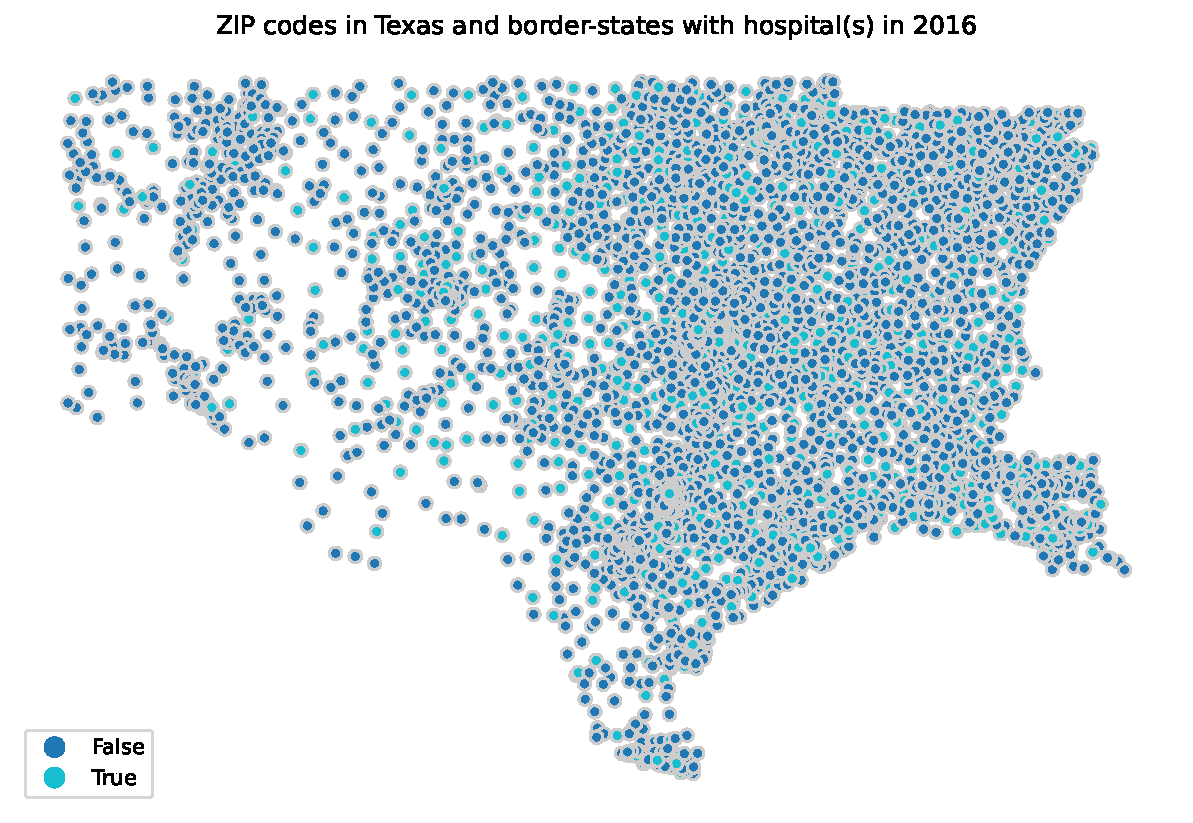
\includegraphics{pset4_files/figure-pdf/cell-30-output-2.pdf}

We merged the GeoDataFrame ``zips\_texas\_borderstates\_centroids'' with
the pos data for short-term hospitals in 2016 merging on Zip codes of
the area , filtering to the ZIP codes whose ``HOSPITAL\_NUM'' is not 0
(those which had at least one hospital in 2016).

\begin{enumerate}
\def\labelenumi{\arabic{enumi}.}
\setcounter{enumi}{3}
\tightlist
\item
  \begin{enumerate}
  \def\labelenumii{\alph{enumii}.}
  \tightlist
  \item
  \end{enumerate}
\end{enumerate}

\begin{Shaded}
\begin{Highlighting}[]
\CommentTok{\# Create a subset of 10 zip codes in TX for testing the calculation of distance}
\NormalTok{zips\_texas\_test }\OperatorTok{=}\NormalTok{ zips\_texas\_centroids.head(}\DecValTok{10}\NormalTok{)}

\CommentTok{\# Start timer}
\NormalTok{start }\OperatorTok{=}\NormalTok{ time.time()}

\CommentTok{\# Join the dataframes}
\NormalTok{join\_test }\OperatorTok{=}\NormalTok{ gpd.sjoin\_nearest(}
\NormalTok{    zips\_texas\_test,}
\NormalTok{    zips\_withhospital\_centroids,}
\NormalTok{    how }\OperatorTok{=} \StringTok{"inner"}\NormalTok{,}
\NormalTok{    distance\_col }\OperatorTok{=} \StringTok{"distance"}
\NormalTok{)}

\CommentTok{\# Find out nearest distance for each TX ZIP code}
\NormalTok{join\_test\_result }\OperatorTok{=}\NormalTok{ join\_test.loc[join\_test.groupby(}\StringTok{"ZCTA5\_left"}\NormalTok{)[}\StringTok{"distance"}\NormalTok{].idxmin()]}

\CommentTok{\# Count the lap time}
\NormalTok{time\_count }\OperatorTok{=}\NormalTok{ time.time() }\OperatorTok{{-}}\NormalTok{ start}

\CommentTok{\# Show the lap time once the row number is correct}
\BuiltInTok{print}\NormalTok{(}\StringTok{"This time, to join the datasets, it took approximately"}\NormalTok{,}
 \BuiltInTok{round}\NormalTok{(time\_count, }\DecValTok{2}\NormalTok{), }\StringTok{"seconds."}\NormalTok{)}

\NormalTok{time\_estimate }\OperatorTok{=}\NormalTok{ (time\_count }\OperatorTok{*} \DecValTok{1935} \OperatorTok{/} \DecValTok{10}\NormalTok{)}

\BuiltInTok{print}\NormalTok{(}\SpecialStringTok{f"As there are 1935 ZIP codes in Texas, we can estimate that it would take approximately }\SpecialCharTok{\{}\BuiltInTok{round}\NormalTok{(time\_count, }\DecValTok{2}\NormalTok{)}\SpecialCharTok{\}}\SpecialStringTok{ * 1935 / 10 = }\SpecialCharTok{\{}\BuiltInTok{round}\NormalTok{(time\_estimate, }\DecValTok{2}\NormalTok{)}\SpecialCharTok{\}}\SpecialStringTok{ seconds."}\NormalTok{)}
\end{Highlighting}
\end{Shaded}

\begin{verbatim}
This time, to join the datasets, it took approximately 0.04 seconds.
As there are 1935 ZIP codes in Texas, we can estimate that it would take approximately 0.04 * 1935 / 10 = 7.71 seconds.
\end{verbatim}

\begin{verbatim}
b.
\end{verbatim}

\begin{Shaded}
\begin{Highlighting}[]
\CommentTok{\# Start timer}
\NormalTok{start }\OperatorTok{=}\NormalTok{ time.time()}

\CommentTok{\# Join the dataframes}
\NormalTok{join\_tx }\OperatorTok{=}\NormalTok{ gpd.sjoin\_nearest(}
\NormalTok{    zips\_texas\_centroids,}
\NormalTok{    zips\_withhospital\_centroids,}
\NormalTok{    how}\OperatorTok{=}\StringTok{"right"}\NormalTok{,}
\NormalTok{    distance\_col}\OperatorTok{=}\StringTok{"distance"}
\NormalTok{)}

\CommentTok{\# Find out nearest distance for each TX ZIP code}
\NormalTok{join\_tx\_min }\OperatorTok{=}\NormalTok{ join\_tx.loc[join\_tx.groupby(}\StringTok{"ZCTA5\_left"}\NormalTok{)[}\StringTok{"distance"}\NormalTok{].idxmin()]}

\CommentTok{\# Count the lap time}
\NormalTok{time\_count }\OperatorTok{=}\NormalTok{ time.time() }\OperatorTok{{-}}\NormalTok{ start}

\CommentTok{\# Show the lap time once the row number is correct}
\BuiltInTok{print}\NormalTok{(}\StringTok{"To join the datasets, it took approximately"}\NormalTok{,}
      \BuiltInTok{round}\NormalTok{(time\_count, }\DecValTok{2}\NormalTok{), }\StringTok{"seconds, which is the quite same level as the test, against our estimation above."}\NormalTok{)}
\end{Highlighting}
\end{Shaded}

\begin{verbatim}
To join the datasets, it took approximately 0.06 seconds, which is the quite same level as the test, against our estimation above.
\end{verbatim}

\begin{verbatim}
c. As the .prj file notes, its unit is a degree (of latitude). A degree of latitude is constantly apploximately convertible to 69 miles, while longitude varies depend on the location, but still maximum about 69 miles.(https://www.thoughtco.com/degree-of-latitude-and-longitude-distance-4070616)

Thus, when interpret the dataset according to the .prj file, it would be suitable to estimate 1 degree = 69 miles.
\end{verbatim}

\begin{enumerate}
\def\labelenumi{\arabic{enumi}.}
\setcounter{enumi}{4}
\item
  \begin{enumerate}
  \def\labelenumii{\alph{enumii}.}
  \item
    The unit is a degree.
  \item
  \end{enumerate}
\end{enumerate}

\begin{Shaded}
\begin{Highlighting}[]
\CommentTok{\# Summarize average distance from the nearest hospital (by ZIP code where the hospital locates) for each ZIP code}
\NormalTok{join\_tx\_avg }\OperatorTok{=}\NormalTok{ join\_tx.groupby(}\StringTok{"ZCTA5\_left"}\NormalTok{)[}\StringTok{"distance"}\NormalTok{].agg(}
    \StringTok{"mean"}\NormalTok{).reset\_index(name}\OperatorTok{=}\StringTok{"distance"}\NormalTok{)}

\CommentTok{\# Convert to mile}
\NormalTok{join\_tx\_avg[}\StringTok{"distance"}\NormalTok{] }\OperatorTok{=}\NormalTok{ join\_tx\_avg[}\StringTok{"distance"}\NormalTok{] }\OperatorTok{*} \DecValTok{69}

\NormalTok{avg\_join\_tx\_avg }\OperatorTok{=}\NormalTok{ join\_tx\_avg[}\StringTok{"distance"}\NormalTok{].mean()}

\BuiltInTok{print}\NormalTok{(avg\_join\_tx\_avg)}
\end{Highlighting}
\end{Shaded}

\begin{verbatim}
1.8753916211405324
\end{verbatim}

\begin{verbatim}
    This intuitively makes sense.

c.
\end{verbatim}

\begin{Shaded}
\begin{Highlighting}[]
\CommentTok{\# Merge the dataframes}
\NormalTok{zips\_texas\_centroids\_merge }\OperatorTok{=}\NormalTok{ zips\_texas\_centroids.merge(}
\NormalTok{    join\_tx\_avg,}
\NormalTok{    left\_on}\OperatorTok{=}\StringTok{"ZCTA5"}\NormalTok{,}
\NormalTok{    right\_on}\OperatorTok{=}\StringTok{"ZCTA5\_left"}\NormalTok{,}
\NormalTok{    how}\OperatorTok{=}\StringTok{"right"}
\NormalTok{)}

\CommentTok{\# Plot the number of hospital in TX on the map}
\NormalTok{zips\_texas\_centroids\_merge.plot(column}\OperatorTok{=}\StringTok{"distance"}\NormalTok{, linewidth}\OperatorTok{=}\FloatTok{0.5}\NormalTok{,}
\NormalTok{                                edgecolor}\OperatorTok{=}\StringTok{"0.8"}\NormalTok{, cmap}\OperatorTok{=}\StringTok{"OrRd"}\NormalTok{, legend}\OperatorTok{=}\VariableTok{True}\NormalTok{, figsize}\OperatorTok{=}\NormalTok{(}\DecValTok{10}\NormalTok{, }\DecValTok{10}\NormalTok{))}

\NormalTok{plt.axis(}\StringTok{"off"}\NormalTok{)}
\NormalTok{plt.title(}
    \StringTok{"Average Distance to the Nearest Hospitals Hospitals by ZIP code in Texas(mil))"}\NormalTok{)}
\NormalTok{plt.show}
\end{Highlighting}
\end{Shaded}

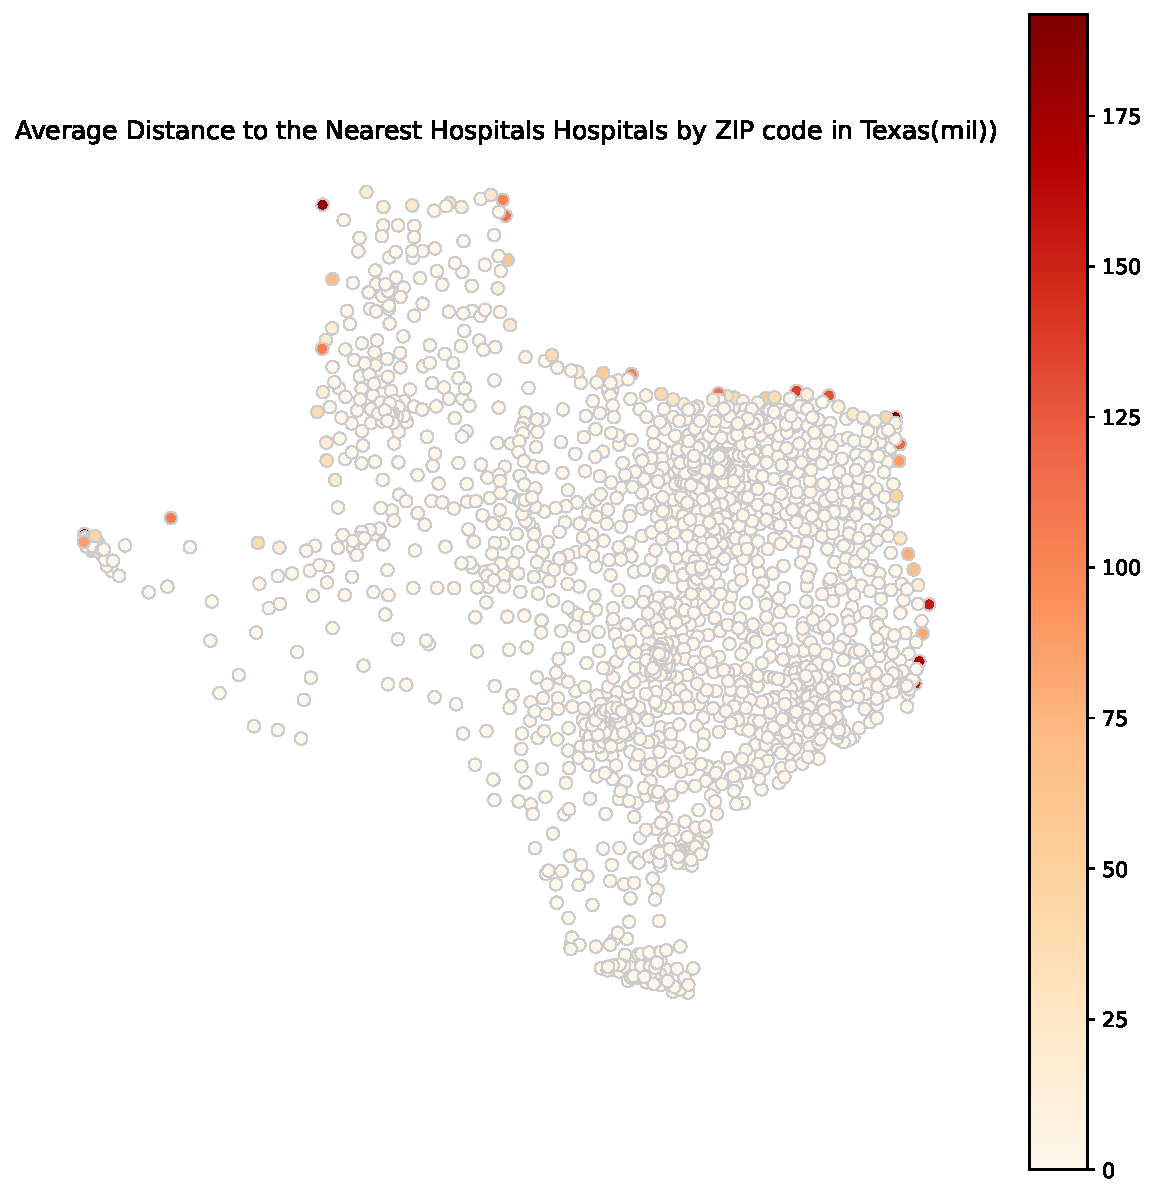
\includegraphics{pset4_files/figure-pdf/cell-34-output-1.pdf}

\subsection{Effects of closures on access in Texas (15
pts)}\label{effects-of-closures-on-access-in-texas-15-pts}

\begin{enumerate}
\def\labelenumi{\arabic{enumi}.}
\tightlist
\item
\end{enumerate}

\begin{Shaded}
\begin{Highlighting}[]
\CommentTok{\# Subset the appended dataset}
\NormalTok{df\_pos\_append[}\StringTok{"ZIP\_CD"}\NormalTok{] }\OperatorTok{=}\NormalTok{ df\_pos\_append[}\StringTok{"ZIP\_CD"}\NormalTok{].astype(}\BuiltInTok{int}\NormalTok{)}
\NormalTok{df\_pos\_append\_tx }\OperatorTok{=}\NormalTok{ df\_pos\_append[(df\_pos\_append[}\StringTok{"ZIP\_CD"}\NormalTok{] }\OperatorTok{\textgreater{}=} \DecValTok{75000}\NormalTok{) }\OperatorTok{\&}\NormalTok{ (}
\NormalTok{    df\_pos\_append[}\StringTok{"ZIP\_CD"}\NormalTok{] }\OperatorTok{\textless{}} \DecValTok{80000}\NormalTok{)]}

\CommentTok{\# Summarize the number of directly affected zip codes}
\NormalTok{summary\_direct }\OperatorTok{=}\NormalTok{ df\_pos\_append\_tx[df\_pos\_append\_tx[}\StringTok{"PGM\_TRMNTN\_CD"}\NormalTok{] }\OperatorTok{!=} \DecValTok{0}\NormalTok{].groupby(}
\NormalTok{    [}\StringTok{"ZIP\_CD"}\NormalTok{, }\StringTok{"FAC\_NAME"}\NormalTok{]).size().reset\_index()}

\NormalTok{summary\_direct }\OperatorTok{=}\NormalTok{ summary\_direct.groupby(}\StringTok{"ZIP\_CD"}\NormalTok{).size().reset\_index()}
\NormalTok{summary\_direct.columns }\OperatorTok{=}\NormalTok{ [}\StringTok{"ZIP code"}\NormalTok{, }\StringTok{"Number of closures"}\NormalTok{]}

\BuiltInTok{print}\NormalTok{(summary\_direct)}
\end{Highlighting}
\end{Shaded}

\begin{verbatim}
     ZIP code  Number of closures
0       75010                   1
1       75020                   2
2       75041                   1
3       75042                   3
4       75051                   2
..        ...                 ...
339     79901                   1
340     79902                   7
341     79904                   1
342     79915                   1
343     79925                   1

[344 rows x 2 columns]
\end{verbatim}

\begin{enumerate}
\def\labelenumi{\arabic{enumi}.}
\setcounter{enumi}{1}
\tightlist
\item
\end{enumerate}

\begin{Shaded}
\begin{Highlighting}[]
\CommentTok{\# Merge the summary to the GeoDataFrame}
\NormalTok{df\_shp\_tx\_merge }\OperatorTok{=}\NormalTok{ df\_shp\_tx\_merge.merge(}
\NormalTok{    summary\_direct,}
\NormalTok{    left\_on}\OperatorTok{=}\StringTok{"ZCTA5"}\NormalTok{,}
\NormalTok{    right\_on}\OperatorTok{=}\StringTok{"ZIP code"}\NormalTok{,}
\NormalTok{    how}\OperatorTok{=}\StringTok{"outer"}
\NormalTok{)}

\NormalTok{df\_shp\_tx\_merge[}\StringTok{"DIRECT"}\NormalTok{] }\OperatorTok{=}\NormalTok{ df\_shp\_tx\_merge[}\StringTok{"Number of closures"}\NormalTok{].}\BuiltInTok{apply}\NormalTok{(}
\NormalTok{    pd.isna)}

\CommentTok{\# Dissolve the GeoDataFrame by the parameter for directly affected ZIP codes}
\NormalTok{dissolved }\OperatorTok{=}\NormalTok{ df\_shp\_tx\_merge[[}\StringTok{"ZCTA5"}\NormalTok{, }\StringTok{"geometry"}\NormalTok{, }\StringTok{"DIRECT"}\NormalTok{]].dissolve(}
\NormalTok{    by}\OperatorTok{=}\StringTok{"DIRECT"}\NormalTok{, aggfunc}\OperatorTok{=}\StringTok{"sum"}\NormalTok{).reset\_index()}
\NormalTok{dissolved}

\CommentTok{\# Plot a choropleth of directly affected ZIP codes}
\NormalTok{dissolved.plot(column}\OperatorTok{=}\StringTok{"DIRECT"}\NormalTok{, linewidth}\OperatorTok{=}\DecValTok{1}\NormalTok{, edgecolor}\OperatorTok{=}\StringTok{"0.8"}\NormalTok{,}
\NormalTok{               legend}\OperatorTok{=}\VariableTok{True}\NormalTok{, figsize}\OperatorTok{=}\NormalTok{(}\DecValTok{10}\NormalTok{, }\DecValTok{10}\NormalTok{))}

\NormalTok{plt.axis(}\StringTok{"off"}\NormalTok{)}
\NormalTok{plt.title(}\StringTok{"Directly Affected ZIP codes in Texas"}\NormalTok{)}
\NormalTok{plt.show}
\end{Highlighting}
\end{Shaded}

\includegraphics{pset4_files/figure-pdf/cell-36-output-1.pdf}

\begin{Shaded}
\begin{Highlighting}[]
\CommentTok{\# Count the number of directly affected ZIP codes}
\BuiltInTok{print}\NormalTok{(}\BuiltInTok{len}\NormalTok{(summary\_direct))}
\end{Highlighting}
\end{Shaded}

\begin{verbatim}
344
\end{verbatim}

There are 344 directly affected zip codes in Texas.

\begin{enumerate}
\def\labelenumi{\arabic{enumi}.}
\setcounter{enumi}{2}
\tightlist
\item
\end{enumerate}

\begin{Shaded}
\begin{Highlighting}[]
\CommentTok{\# Create a GeoDataFrame of the directly affected zip codes}
\NormalTok{direct\_zips }\OperatorTok{=}\NormalTok{ dissolved[dissolved[}\StringTok{"DIRECT"}\NormalTok{] }\OperatorTok{==} \DecValTok{1}\NormalTok{]}

\CommentTok{\# Create a 10{-}mile buffer around direct\_zips}
\NormalTok{buf\_degree }\OperatorTok{=} \DecValTok{10} \OperatorTok{/} \DecValTok{69}

\NormalTok{buffer\_10 }\OperatorTok{=}\NormalTok{ direct\_zips.copy()}
\NormalTok{buffer\_10[}\StringTok{"geometry"}\NormalTok{] }\OperatorTok{=}\NormalTok{ buffer\_10.geometry.}\BuiltInTok{buffer}\NormalTok{(buf\_degree)}

\CommentTok{\# Spatial join with the overall Texas zip code shapefile}
\NormalTok{indirect\_zips }\OperatorTok{=}\NormalTok{ gpd.sjoin(df\_shp\_tx, buffer\_10,}
\NormalTok{                          how}\OperatorTok{=}\StringTok{"inner"}\NormalTok{, predicate}\OperatorTok{=}\StringTok{"intersects"}\NormalTok{)}

\BuiltInTok{print}\NormalTok{(}\BuiltInTok{len}\NormalTok{(indirect\_zips))}
\end{Highlighting}
\end{Shaded}

\begin{verbatim}
1935
\end{verbatim}

There are 1935 indirectly affected zipcodes in Texas.

\begin{enumerate}
\def\labelenumi{\arabic{enumi}.}
\setcounter{enumi}{3}
\tightlist
\item
\end{enumerate}

\begin{Shaded}
\begin{Highlighting}[]
\NormalTok{fig, ax }\OperatorTok{=}\NormalTok{ plt.subplots()}
\NormalTok{direct\_zips.plot(ax}\OperatorTok{=}\NormalTok{ax, color}\OperatorTok{=}\StringTok{"red"}\NormalTok{, alpha}\OperatorTok{=}\FloatTok{0.7}\NormalTok{, label}\OperatorTok{=}\StringTok{"Direct"}\NormalTok{).set\_axis\_off()}
\NormalTok{buffer\_10.plot(ax}\OperatorTok{=}\NormalTok{ax, color}\OperatorTok{=}\StringTok{"purple"}\NormalTok{, alpha}\OperatorTok{=}\FloatTok{0.5}\NormalTok{,}
\NormalTok{               label}\OperatorTok{=}\StringTok{"10{-}mile"}\NormalTok{).set\_axis\_off()}
\NormalTok{indirect\_zips.plot(ax}\OperatorTok{=}\NormalTok{ax, color}\OperatorTok{=}\StringTok{"blue"}\NormalTok{, alpha}\OperatorTok{=}\FloatTok{0.3}\NormalTok{, label}\OperatorTok{=}\StringTok{"Indirect"}\NormalTok{)}

\NormalTok{plt.show()}
\end{Highlighting}
\end{Shaded}

\includegraphics{pset4_files/figure-pdf/cell-39-output-1.pdf}

\subsection{Reflecting on the exercise (10
pts)}\label{reflecting-on-the-exercise-10-pts}

(Partner 1: Hiro) One possible reason for the number of active hospitals
in a zip code to not decrease is the opening of a totally new hospital.
The ``first-pass'' method does not distinguish between a potential
merger (where the hospital name/address is the same) and the opening of
a totally new hospital. In such a case, a valid closure would not be
counted. To get a more accurate confirmation of hospital closures in
using the ``first-pass'' method, we could also look at a secondary
datapoint such as address which is harder to change compared to hospital
name. Another possible way is to add more details in the termination
status column. For example, a code specific for mergers could be added
that would make it easier to filter~these~entries.

(Partner 2: Luis)

As our research design simply focus on geographical distance (impact of
closures to those who arewithin the same ZIP codes, or within 10 miles
distance), it might not reflect the real usage of hospitals by
residents. For instance, as we ignore their preferences or genres of
hospitals correlated to diseases categories, thus some people might have
been using specific hospitals which is not the nearest ones from their
place. Also, we ignore the transportation and the concentration of
hospitals (hospitals might be originally concentrated on large city and
frequently used by residents living broadly around the city). To improve
this research from those reflection, we can merge additional attributes
to the GeoDataFrame, such as the population for each ZIP code, the
concentration of hospitals (= number of hospitals per ZIP code), and if
possible, parameter of whether major transportation (railway, bus,
highway) exists in the ZIP~code~or~not.




\end{document}
